\chapter*{Установка НЕВОД-ДЕКОР}
\addcontentsline{toc}{chapter}{Установка НЕВОД-ДЕКОР}
\label{ch:intro}

Координатно-трековый детектор ДЕКОР \cite{barbashina2000coordinate} представляет собой крупномасштабную установку, специально предназначенную для изучения мюонов космического излучения на поверхности Земли в широком диапазоне зенитных углов вплоть до горизонта. Установка состоит из 8 сборок-супермодулей (СМ00 – СМ07) по 8 слоев пластиковых камер из стримерных трубок, общая площадь ~ 70 м$^2$, 32768 каналов регистрации. По данным детектора ДЕКОР можно найти количество треков в группе мюонов и определить ее направление. Точность локализации трека в одном СМ лучше 1 см, а точность оценки направления – лучше $1\degree$. Супермодули детектора ДЕКОР расположены в галереях здания с трех сторон от черенковского водного детектора (ЧВД) НЕВОД объемом 2000 м$^3$. На рис. 1 изображена схема установки НЕВОД-ДЕКОР (а) и структура супермодуля детектора ДЕКОР (б).

\begin{figure}[ht]
	\centering
\hspace*{\fill}%
	\begin{subfigure}[b]{0.7\textwidth}
        \centering
		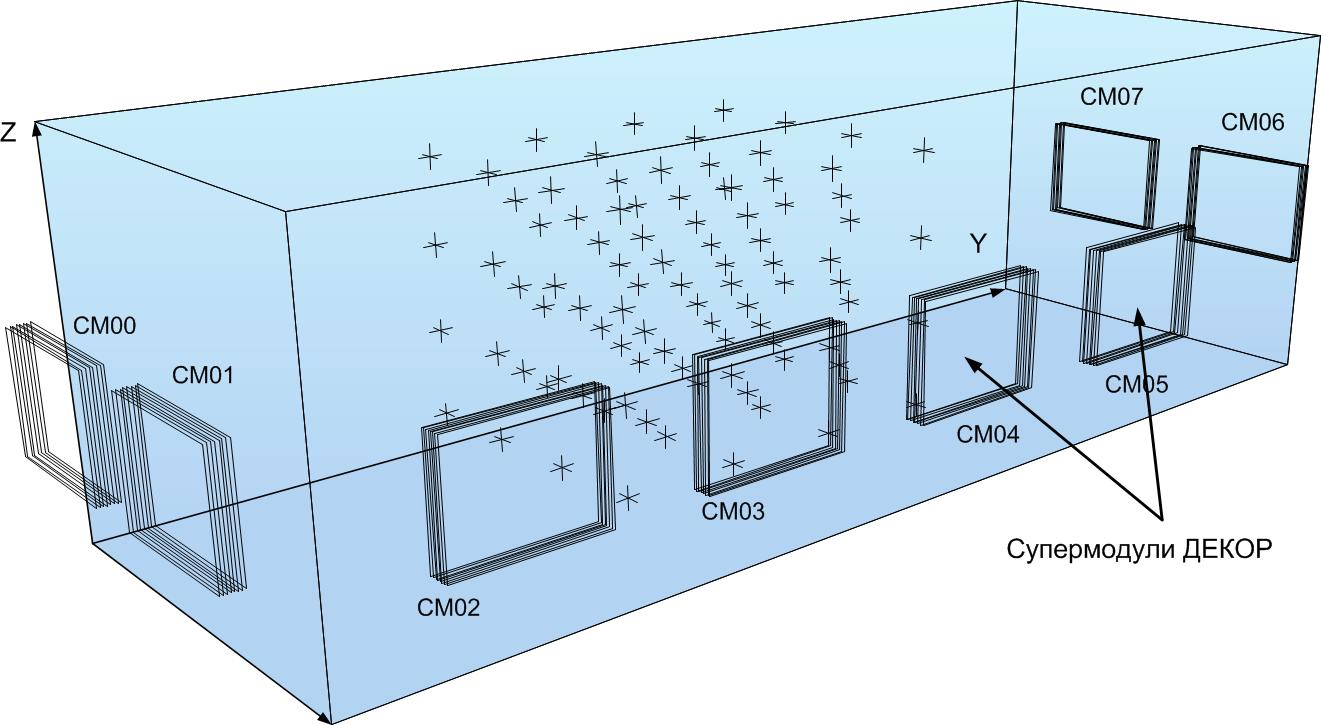
\includegraphics[height=10cm,keepaspectratio]{DECOR_1}
		\caption{}
		\label{fig:DECOR_1}
	\end{subfigure}
\hfill
	\begin{subfigure}[b]{0.29\textwidth}
        \centering
		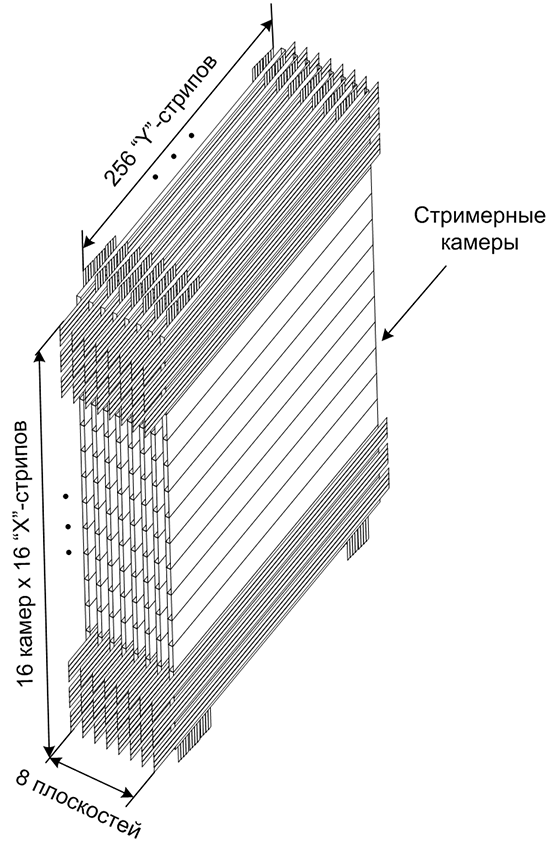
\includegraphics[height=10cm,keepaspectratio]{DECOR_2}
        \caption{}
		\label{fig:DECOR_2}
	\end{subfigure}
\hspace*{\fill}%
	\caption{Общая схема установки НЕВОД-ДЕКОР (a) и структура супермодуля детектора ДЕКОР (б)}
	\label{fig:tiger}
\end{figure}

НЕВОД \cite{petrukhin2015cherenkov} предназначен для изучения всех основных компонент космических лучей на поверхности Земли и состоит из 91 квазисферического измерительного модуля (КСМ), которые расположены в узлах пространственной решетки. Фактически решетка сформирована из 25 вертикальных гирлянд по 3 или 4 КСМ. Каждый КСМ состоит из 6 фотоумножителей с плоским фотокатодом, ориентированных вдоль осей ортогональной системы координат. Такая конструкция обеспечивает практически одинаковую эффективность регистрации черенковского излучения, приходящего с любого направления. Широкий динамический диапазон измерений каждого ФЭУ (от 1 до $10^5$ фотоэлектронов) позволяет проводить калориметрические исследования, в частности, измерять энерговыделения групп мюонов. 
Для калибровки спектрометрических трактов черенковского водного калориметра НЕВОД во время длительных экспериментальных серий, а также для исследований широких атмосферных
ливней энергетическом диапазоне первичных частиц от 0.1 до 100 ПэВ используется система калибровочных телескопов (СКТ). Система калибровочных телескопов (СКТ) состоит из 80 сцинтилляционных детекторов. Сорок детекторов расположены на крышке и сорок – на дне водного бассейна ЧВК НЕВОД (верхняя и нижняя плоскости).

\endinput